\documentclass[11pt,a4paper]{article}

\usepackage[margin=2.3cm]{geometry}
\usepackage[T1]{fontenc}
\usepackage{lmodern}
\usepackage{microtype}
\usepackage{amsmath,amssymb}
\usepackage{booktabs}
\usepackage{tabularx}
\usepackage{enumitem}
\usepackage{caption}
\usepackage{placeins}
\usepackage{xcolor}
\usepackage{tikz}
\usetikzlibrary{arrows.meta,positioning,calc,fit,backgrounds,shapes.geometric,decorations.pathreplacing}
\usepackage[hidelinks]{hyperref}

\setlist{itemsep=2pt,topsep=4pt}
\newcommand{\code}[1]{\texttt{#1}}
\newcommand{\vect}[1]{\mathbf{#1}}
\newcolumntype{L}{>{\raggedright\arraybackslash}X}
\tikzset{
  box/.style={draw, rounded corners=2pt, align=center, font=\small, minimum height=8mm, inner sep=3pt, fill=white},
  data/.style={box, fill=gray!12},
  model/.style={box, fill=blue!8},
  arr/.style={-{Stealth[length=2mm]}, thick},
  note/.style={font=\footnotesize\itshape, align=center, text=black!70}}

\title{Prerequisites for the Semantic Embedding Report:\\[2pt]
\large Gaussian Splats, CLIP, DINOv2, SAM, the Lift and FMGS --- what each does and how}
\author{Suhan --- Team Radiance, Department of Computer Science and Engineering,\\University of Moratuwa}
\date{8 October 2026}

\begin{document}
\maketitle

\begin{abstract}
This companion note explains, at an abstract level, the building blocks used by our semantic layer: the 3D
Gaussian Splat it is attached to, the three 2D foundation models that supply features (CLIP for language, DINOv2
for object structure, SAM for object outlines), the relevancy score that turns a phrase into a per-point score,
and the two ways of attaching 2D features to a 3D splat (the training-free \emph{lift} and the trained
\emph{FMGS} feature field). It contains no results; the main report (\code{semantic\_embedding\_report.tex}) builds
on these ideas.
\end{abstract}

\tableofcontents

%=======================================================================================
\section{The problem in one picture}
%=======================================================================================

We have a photo-realistic 3D model of a room (a \emph{Gaussian splat}) and the photos it was made from. We want to
type ``red cup'' and get back the 3D position of the red cup, so that a drone course can end in front of it. The
splat itself knows only colour and geometry; it has no idea what a cup is. So we borrow understanding from 2D image
models, which are trained on hundreds of millions of images, and transfer what they see in each photo onto the 3D
points (Figure~\ref{fig:big}).

\begin{figure}[ht]
\centering
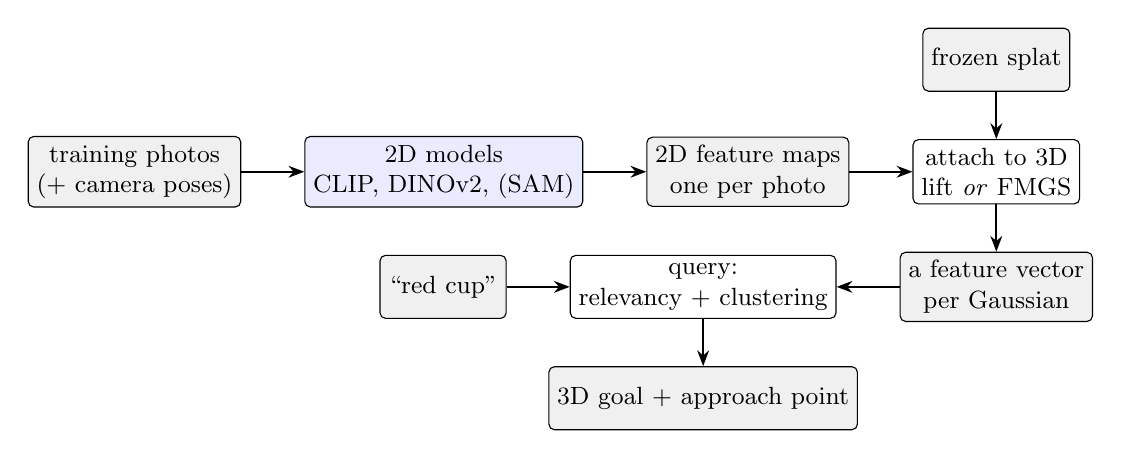
\begin{tikzpicture}[node distance=6mm and 8mm]
  \node[data] (photos) {training photos\\(+ camera poses)};
  \node[model, right=of photos] (models) {2D models\\CLIP, DINOv2, (SAM)};
  \node[data, right=of models] (maps) {2D feature maps\\one per photo};
  \node[box, right=of maps] (attach) {attach to 3D\\lift \emph{or} FMGS};
  \node[data, below=of attach] (table) {a feature vector\\per Gaussian};
  \node[box, left=of table] (query) {query:\\relevancy + clustering};
  \node[data, left=of query] (text) {``red cup''};
  \node[data, below=of query] (goal) {3D goal + approach point};
  \node[data, above=of attach] (splat) {frozen splat};
  \draw[arr] (photos) -- (models); \draw[arr] (models) -- (maps); \draw[arr] (maps) -- (attach);
  \draw[arr] (splat) -- (attach); \draw[arr] (attach) -- (table); \draw[arr] (table) -- (query);
  \draw[arr] (text) -- (query); \draw[arr] (query) -- (goal);
\end{tikzpicture}
\caption{The overall idea: 2D models see the photos, their features are transferred onto the 3D splat, and a phrase is
compared against those features.}
\label{fig:big}
\end{figure}

%=======================================================================================
\section{3D Gaussian Splatting}
%=======================================================================================

\paragraph{What it is.} A 3D Gaussian splat~\cite{3dgs} represents a scene as hundreds of thousands of small,
semi-transparent, coloured ellipsoids (``Gaussians''). Each Gaussian $i$ has a centre $\vect{x}_i$, an orientation
and three axis lengths (its shape), an opacity $o_i$ and a view-dependent colour. Our backroom scene has 532{,}361
Gaussians.

\paragraph{How an image is rendered.} For a camera, every Gaussian is projected to a 2D ellipse on the image. For each
pixel, the ellipses covering it are sorted front to back and their colours are \emph{alpha-blended}:
\begin{equation}
  C(p) = \sum_{i} \underbrace{\alpha_i(p) \prod_{j<i}\bigl(1-\alpha_j(p)\bigr)}_{w_i(p)} \, c_i ,
\end{equation}
where $\alpha_i(p)$ is the Gaussian's opacity times its 2D footprint at pixel $p$, and the product is the light
that survives the Gaussians in front. The quantity $w_i(p)$ --- the \emph{blend weight} --- says how much Gaussian
$i$ contributes to pixel $p$. Two facts matter for us:
\begin{enumerate}
  \item \textbf{Any per-Gaussian vector can be rendered}, not just colour: replace $c_i$ by a feature vector
        $\vect{f}_i$ and the same formula produces a feature image. The rasteriser we use (gsplat~1.0.0) can
        render up to 512 channels forward, but only 32 channels when gradients are needed, so features are rendered
        in 32-channel chunks.
  \item \textbf{Rendering is linear in the per-Gaussian values}, which is what makes the lift (Section~\ref{sec:lift})
        possible without any training.
\end{enumerate}

\paragraph{Training a splat.} The Gaussians are optimised so that renders match the photos (FiGS uses nerfstudio's
\code{splatfacto}, 30{,}000 steps). It also refines each camera's pose a little. In our work the splat is
\textbf{frozen}: its Gaussians are never changed again, because drone courses, cached renders and trained policies all
depend on them.

\begin{figure}[ht]
\centering
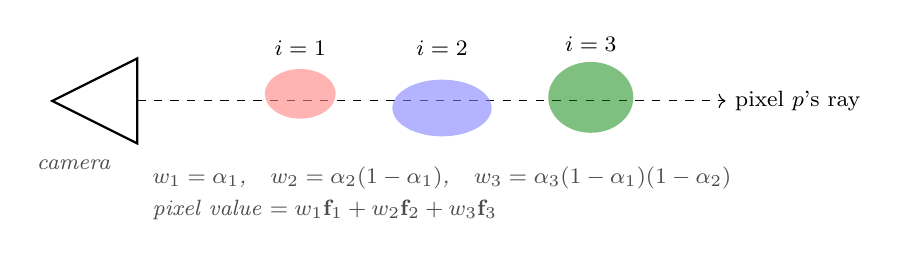
\begin{tikzpicture}[scale=0.9]
  % camera
  \draw[thick] (0,0) -- (1.2,0.6) -- (1.2,-0.6) -- cycle; \node[note] at (0.3,-0.9) {camera};
  % ray
  \draw[dashed, ->] (1.2,0) -- (9.5,0) node[right, font=\footnotesize] {pixel $p$'s ray};
  % gaussians
  \fill[red!50, opacity=0.6] (3.5,0.1) ellipse (0.5 and 0.35); \node[font=\footnotesize] at (3.5,0.75) {$i=1$};
  \fill[blue!50, opacity=0.6] (5.5,-0.1) ellipse (0.7 and 0.4); \node[font=\footnotesize] at (5.5,0.75) {$i=2$};
  \fill[green!50!black, opacity=0.5] (7.6,0.05) ellipse (0.6 and 0.5); \node[font=\footnotesize] at (7.6,0.8) {$i=3$};
  \node[note, align=left] at (5.5,-1.3) {$w_1 = \alpha_1$,\quad $w_2 = \alpha_2(1-\alpha_1)$,\quad
     $w_3 = \alpha_3(1-\alpha_1)(1-\alpha_2)$\\[2pt] pixel value $= w_1\vect{f}_1 + w_2\vect{f}_2 + w_3\vect{f}_3$};
\end{tikzpicture}
\caption{Alpha blending along one pixel's ray. The blend weight $w_i$ of each Gaussian is how much it contributes to
the pixel; front Gaussians hide the ones behind them.}
\label{fig:blend}
\end{figure}

%=======================================================================================
\section{CLIP: images and text in one space}
%=======================================================================================

\paragraph{What it does.} CLIP~\cite{clip} is a pair of neural networks --- an image encoder and a text encoder ---
trained on hundreds of millions of image--caption pairs so that an image and a caption that describes it map to
nearby unit vectors (high cosine similarity), and unrelated pairs to distant ones. After training, \emph{any} phrase
can be compared with \emph{any} image, without a fixed list of classes: this is what makes our queries
\emph{open-vocabulary}.

\begin{figure}[ht]
\centering
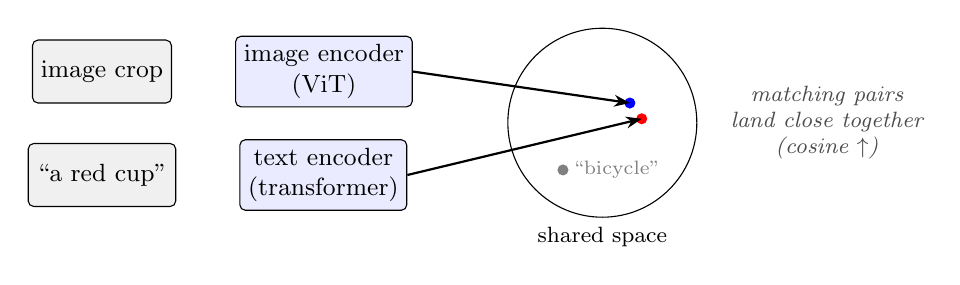
\begin{tikzpicture}[node distance=5mm and 8mm]
  \node[data] (img) {image crop};
  \node[model, right=of img] (ienc) {image encoder\\(ViT)};
  \node[data, below=of img] (txt) {``a red cup''};
  \node[model, right=of txt] (tenc) {text encoder\\(transformer)};
  \node[circle, draw, right=12mm of ienc, yshift=-6.5mm, minimum size=2.4cm, label=below:{\footnotesize shared space}] (sp) {};
  \fill[blue] ($(sp.center)+(0.35,0.25)$) circle (2pt) coordinate (pi);
  \fill[red] ($(sp.center)+(0.5,0.05)$) circle (2pt) coordinate (pt);
  \fill[gray] ($(sp.center)+(-0.5,-0.6)$) circle (2pt) node[right, font=\scriptsize] {``bicycle''};
  \draw[arr] (ienc.east) -- (pi); \draw[arr] (tenc.east) -- (pt);
  \node[note, right=3mm of sp] {matching pairs\\land close together\\(cosine $\uparrow$)};
\end{tikzpicture}
\caption{CLIP maps images and text into one space of unit vectors (512-d for ViT-B/16, 768-d for ViT-L/14).}
\end{figure}

\paragraph{How.} The image encoder is a Vision Transformer (ViT): it cuts a $224\times224$ image into patches
($16\times16$ pixels for ViT-B/16, $14\times14$ for ViT-L/14), processes them with self-attention, and summarises the
whole image into \emph{one} vector. Training uses a contrastive loss: in a batch of $N$ image--caption pairs, each
image must be most similar to its own caption among the $N$. We use OpenCLIP models trained on LAION-2B: ViT-B/16
(512-d) by default and ViT-L/14 (768-d, about 3.5$\times$ the compute) in variant C.

\paragraph{Why it is coarse.} CLIP describes a \emph{whole image} with one vector; it does not say where in the image
things are. To get a per-pixel map we must embed many crops and assign each crop's vector to the pixels it covers.
That is the \textbf{crop pyramid}:
\begin{itemize}
  \item square crops of several sizes (we use 7 scales, from 5\,\% to 50\,\% of the image's short side) slide over the
        photo with half-crop overlap;
  \item each crop is resized to $224\times224$ and embedded;
  \item every crop's vector is written at its centre, giving one coarse grid per scale, and the grids are resampled to
        one common grid (about $71\times40$ cells per photo).
\end{itemize}
Small crops see small objects clearly but lack context; large crops see context but drown small objects. How the
scales are \emph{combined} --- averaged (``Old''), kept separate (variant A), or replaced by object-shaped segments
(variant B) --- is the main subject of the report.

\begin{figure}[ht]
\centering
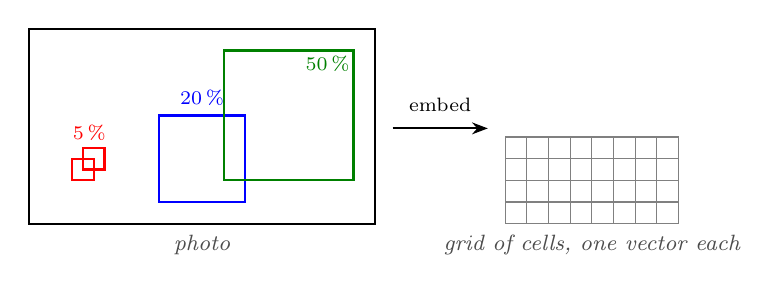
\begin{tikzpicture}[scale=0.55]
  \draw[thick] (0,0) rectangle (8,4.5); \node[note] at (4,-0.5) {photo};
  \draw[red, thick] (1,1) rectangle (1.5,1.5); \draw[red, thick] (1.25,1.25) rectangle (1.75,1.75);
  \draw[blue, thick] (3,0.5) rectangle (5,2.5);
  \draw[green!50!black, thick] (4.5,1) rectangle (7.5,4);
  \node[font=\scriptsize, red] at (1.4,2.1) {5\,\%};
  \node[font=\scriptsize, blue] at (4,2.9) {20\,\%};
  \node[font=\scriptsize, green!50!black] at (6.9,3.7) {50\,\%};
  \begin{scope}[xshift=11cm]
    \foreach \x in {0,...,7} \foreach \y in {0,...,3} \draw[gray] (\x*0.5,\y*0.5) rectangle ++(0.5,0.5);
    \node[note] at (2,-0.5) {grid of cells, one vector each};
  \end{scope}
  \draw[arr] (8.4,2.2) -- (10.6,2.2); \node[font=\scriptsize] at (9.5,2.75) {embed};
\end{tikzpicture}
\caption{The CLIP crop pyramid: overlapping square crops at several scales are embedded and placed on a grid.}
\end{figure}

%=======================================================================================
\section{Relevancy: turning a phrase into a score per point}
%=======================================================================================

A CLIP vector $\vect{f}$ at a point and a phrase's text vector $\vect{t}$ give a cosine similarity, but raw
similarities are not comparable across phrases. LERF~\cite{lerf} therefore compares the phrase against a few
\emph{canonical negatives} (\emph{object, things, stuff, texture}) and asks how much more the point resembles the
phrase than the most similar negative:
\begin{equation}
  r = \min_j \; \sigma\bigl(T\,(\cos(\vect{f}, \vect{t}) - \cos(\vect{f}, \vect{n}_j))\bigr), \qquad T = 10 .
\end{equation}
$r = 0.5$ means ``no preference''; values near 1 mean the point clearly looks like the phrase. Our query keeps
points above a \emph{threshold} relative to the phrase's own peak (with a fixed lower bound, the \emph{floor},
0.55), groups them into 3D clusters, and returns the best cluster's centre. Because $r$ depends on the scale of
CLIP's similarities, the floor is \emph{model-specific}: a different CLIP model needs a different floor (this
is the point of variant C2).

%=======================================================================================
\section{DINOv2: what belongs together}
%=======================================================================================

\paragraph{What it does.} DINOv2~\cite{dinov2} is a Vision Transformer trained \emph{without any labels or text}, by
self-distillation: a ``student'' network sees distorted crops of an image and must produce the same features as a
slowly-updated ``teacher'' network that sees other crops, plus a masked-patch prediction task. The result is a
feature vector for \emph{every patch} ($14\times14$ pixels) in which patches of the same object or material are
similar and object boundaries are sharp.

\paragraph{Why we use it.} DINOv2 knows nothing about words, so it cannot answer a query. But it is dense and
precise where CLIP is coarse, so it is used as a \emph{helper}: in FMGS it teaches the feature field where objects
begin and end (pixel alignment), and in the L-CD query it smooths relevancy within an object and splits candidates
that merge two objects. We use ViT-S/14 (384-d), run on the photo resized to multiples of 14 pixels
($\approx64\times36$ patches).

\begin{table}[ht]
\centering\small
\begin{tabularx}{\linewidth}{@{}lLL@{}}
\toprule
 & CLIP & DINOv2 \\
\midrule
Trained with & image--caption pairs (contrastive) & images only (self-distillation) \\
Output & one vector per image (crop) & one vector per $14\times14$ patch \\
Understands words & yes --- open vocabulary & no \\
Spatial precision & coarse (crop-sized) & sharp (patch-sized, object boundaries) \\
Our use & answers the query & sharpens/organises CLIP (FMGS loss, L-CD) \\
\bottomrule
\end{tabularx}
\caption{The two teachers are complementary.}
\end{table}

%=======================================================================================
\section{SAM: object outlines (used by variants B and B2)}
%=======================================================================================

The Segment Anything Model~\cite{sam} cuts an image into object-shaped masks. Its \emph{automatic mask generator}
places a grid of prompt points over the image ($32\times32$ in our setting), predicts masks for each point, and keeps
the confident, stable, non-duplicate ones. SAM has no notion of words either; in variant B we feed CLIP each
\emph{segment} (its cut-out, background blacked out) instead of square crops, as LangSplat~\cite{langsplat} does, so
that a CLIP vector describes one object rather than a window mixing an object with its surroundings. We use SAM's
ViT-B model.

\begin{figure}[ht]
\centering
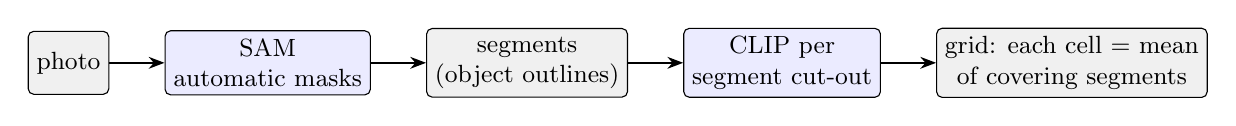
\begin{tikzpicture}[node distance=5mm and 7mm]
  \node[data] (p) {photo};
  \node[model, right=of p] (sam) {SAM\\automatic masks};
  \node[data, right=of sam] (m) {segments\\(object outlines)};
  \node[model, right=of m] (clip) {CLIP per\\segment cut-out};
  \node[data, right=of clip] (g) {grid: each cell = mean\\of covering segments};
  \draw[arr] (p) -- (sam); \draw[arr] (sam) -- (m); \draw[arr] (m) -- (clip); \draw[arr] (clip) -- (g);
\end{tikzpicture}
\caption{Region-level CLIP: SAM gives the outlines, CLIP describes each region.}
\end{figure}

%=======================================================================================
\section{The lift: attaching 2D features to Gaussians without training}
\label{sec:lift}
%=======================================================================================

\paragraph{What it does.} The lift~\cite{occam,ludvig} gives each Gaussian the \emph{weighted average} of the 2D
feature-map values at all the pixels it contributes to, in all training photos, weighted by its blend weight:
\begin{equation}
  \vect{f}_i \;=\; \frac{\sum_{\text{photos } v}\sum_{\text{pixels } p} w_i(v,p)\, F_v(p)}
                         {\sum_{v}\sum_{p} w_i(v,p)} .
\end{equation}
A Gaussian that is clearly visible in a pixel (large $w_i$) takes much of that pixel's feature; one hidden behind
others (small $w_i$) takes little. Gaussians never seen by any photo get no features and are marked \emph{unseen}.

\paragraph{How, cheaply.} Because rendering is linear in the per-Gaussian values, the numerator is exactly the
gradient of $\sum_p \langle \mathrm{render}(\vect{f}), F_v \rangle$ with respect to $\vect{f}$, and the denominator
is the gradient of $\sum_p \mathrm{render}(\vect{1})$. So the whole lift is one backward pass of the rasteriser per
photo and feature chunk --- no optimisation, no hyper-parameters, a few minutes on our GPU.

\begin{figure}[ht]
\centering
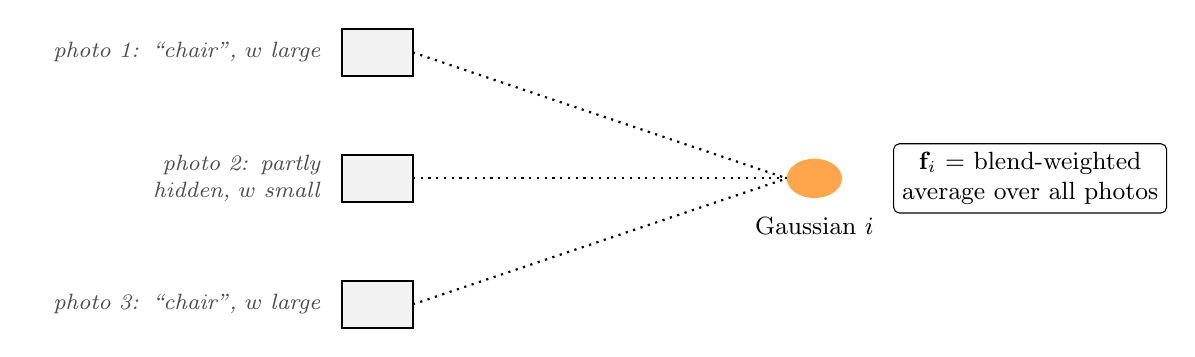
\begin{tikzpicture}
  \fill[orange!70] (6,0) ellipse (0.35 and 0.25) coordinate (G);
  \node[font=\small] at (6,-0.6) {Gaussian $i$};
  \foreach \y/\t in {1.6/{photo 1: ``chair'', $w$ large}, 0/{photo 2: partly hidden, $w$ small}, -1.6/{photo 3: ``chair'', $w$ large}} {
    \draw[thick, fill=gray!10] (0,\y-0.3) rectangle (0.9,\y+0.3);
    \draw[dotted, thick] (0.9,\y) -- (5.65,0);
    \node[note, anchor=east, text width=3.6cm, align=right] at (-0.15,\y) {\t};
  }
  \node[box, anchor=west] at (7,0) {$\vect{f}_i$ = blend-weighted\\average over all photos};
\end{tikzpicture}
\caption{The lift: a Gaussian collects the features of the pixels it is seen in, from every photo.}
\end{figure}

\paragraph{Strengths and limits.} The lift is fast, deterministic and cannot ``invent'' anything: it reproduces the
teacher maps faithfully in 3D (we measured that it loses almost no relevancy). Its quality is therefore bounded by the
2D teacher maps --- coarse in, coarse out --- and it stores one vector per Gaussian per feature (0.7--2.5\,GB per scene).

%=======================================================================================
\section{FMGS: a trained feature field}
%=======================================================================================

\paragraph{What it does.} FMGS~\cite{fmgs} (Foundation Model Gaussian Splatting) does not store a free vector per
Gaussian. It learns a \emph{function} of 3D position --- a neural feature field --- that outputs a CLIP vector and a
DINO vector at any point. The field is evaluated at the Gaussian centres, the result is rendered like colour, and the
rendered maps are compared with the teacher maps of the same photo. Training adjusts only the field (the splat stays
frozen).

\paragraph{How.} The field has two parts:
\begin{itemize}
  \item a \textbf{multi-resolution hash grid}~\cite{instantngp}: 24 grids of increasing resolution (16 to 512 cells per
        side) cover the scene; each grid's corners store small learned vectors (8 numbers) in a hash table. A 3D point
        reads the 8 corners around it in every grid, interpolates, and concatenates the 24 results into a 192-number
        code. Coarse grids describe large regions; fine grids describe detail.
  \item small \textbf{MLP heads} that turn that code into a 512-d CLIP vector and a 384-d DINO vector.
\end{itemize}
The loss has three parts: CLIP rendered vs CLIP teacher (Huber), DINO rendered vs DINO teacher (squared error), and
\emph{pixel alignment}, which asks neighbouring pixels of the rendered CLIP map to be as similar to each other as
DINO says they should be --- transferring DINO's sharp object boundaries to CLIP. After training the field is
evaluated once at every Gaussian centre (``baking'') to produce the same per-Gaussian table as the lift.

\begin{figure}[ht]
\centering
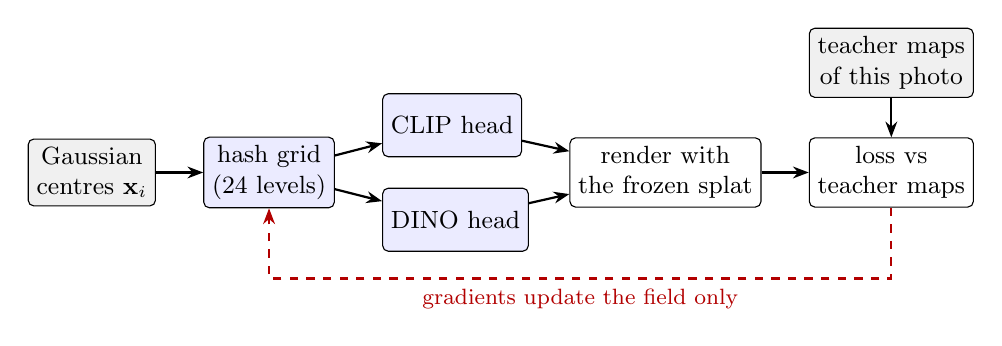
\begin{tikzpicture}[node distance=5mm and 6mm]
  \node[data] (x) {Gaussian\\centres $\vect{x}_i$};
  \node[model, right=of x] (hg) {hash grid\\(24 levels)};
  \node[model, right=of hg, yshift=6mm] (hc) {CLIP head};
  \node[model, right=of hg, yshift=-6mm] (hd) {DINO head};
  \node[box, right=of hc, yshift=-6mm] (r) {render with\\the frozen splat};
  \node[box, right=of r] (l) {loss vs\\teacher maps};
  \node[data, above=of l] (t) {teacher maps\\of this photo};
  \draw[arr] (x) -- (hg); \draw[arr] (hg) -- (hc); \draw[arr] (hg) -- (hd);
  \draw[arr] (hc) -- (r); \draw[arr] (hd) -- (r); \draw[arr] (r) -- (l); \draw[arr] (t) -- (l);
  \draw[arr, dashed, red!70!black] (l.south) -- ++(0,-0.9) -| node[pos=0.25, below, font=\footnotesize] {gradients update the field only} (hg.south);
\end{tikzpicture}
\caption{One FMGS training step: the field predicts features at the Gaussians, they are rendered, compared with the
photo's teacher maps, and only the field is updated.}
\end{figure}

\paragraph{Strengths and limits.} Because nearby points share hash-grid entries, the field \emph{smooths} and can
fill in Gaussians seen in few photos, and it can answer arbitrary 3D points, not just Gaussian centres. But it is a
trained approximation of the teacher maps: limited capacity, a loss dominated by its largest term, and a training run
of 25--45 minutes on our GPU. When the teacher maps contain something misleading (for example zero vectors where SAM
found nothing), the field learns it faithfully.

%=======================================================================================
\section{Glossary}
%=======================================================================================

\begin{table}[ht]
\centering\small
\begin{tabularx}{\linewidth}{@{}lL@{}}
\toprule
Term & Meaning \\
\midrule
Teacher map & A 2D feature map (CLIP or DINO) computed from one training photo; the ``teacher'' that the 3D features learn from or are averaged from. \\
Crop pyramid & CLIP embeddings of square crops at several scales, placed on a grid. \\
Scale group & Variant A: crops of similar size (small / medium / large) averaged together, kept separate from other groups. \\
Segment level & Variant B2: SAM segments of similar area (parts / objects / regions), one map each. \\
Table & The per-Gaussian result: CLIP (and DINO) vector, blend weight, geometry; rows in the same order as Galley's \code{.splat}. \\
Relevancy & LERF's per-point score of a phrase versus canonical negatives; 0.5 = indifferent. \\
Floor & The lowest relevancy that can ever count as a match (0.55 for ViT-B/16). \\
Peak & The mean of the 100 highest relevancies of a query; the threshold is set halfway between floor and peak. \\
Hit & The top candidate's box (grown by 0.3\,m) contains an annotated instance, or its centre is within 0.75\,m of one. \\
L-C / L-CD & Lift table, queried with CLIP only / with DINO smoothing and splitting at query time. \\
F-C / F-CD & FMGS trained on CLIP alone / with its paper losses (CLIP + DINO + pixel alignment). \\
AUROC & Probability that a present object's peak relevancy exceeds an absent object's; 1 = perfect separation. \\
\bottomrule
\end{tabularx}
\end{table}

\begin{thebibliography}{9}
\bibitem{3dgs} B.~Kerbl, G.~Kopanas, T.~Leimk\"uhler, G.~Drettakis.
  \emph{3D Gaussian Splatting for Real-Time Radiance Field Rendering.} ACM TOG 2023.
\bibitem{clip} A.~Radford et al. \emph{Learning Transferable Visual Models From Natural Language Supervision.} ICML 2021.
\bibitem{dinov2} M.~Oquab et al. \emph{DINOv2: Learning Robust Visual Features without Supervision.} TMLR 2024.
\bibitem{sam} A.~Kirillov et al. \emph{Segment Anything.} ICCV 2023.
\bibitem{lerf} J.~Kerr, C.~M.~Kim, K.~Goldberg, A.~Kanazawa, M.~Tancik.
  \emph{LERF: Language Embedded Radiance Fields.} ICCV 2023.
\bibitem{langsplat} M.~Qin, W.~Li, J.~Zhou, H.~Wang, H.~Pfister. \emph{LangSplat: 3D Language Gaussian Splatting.} CVPR 2024.
\bibitem{fmgs} X.~Zuo, P.~Samangouei, Y.~Zhou, Y.~Di, M.~Li.
  \emph{FMGS: Foundation Model Embedded 3D Gaussian Splatting for Holistic 3D Scene Understanding.} IJCV 2024.
\bibitem{instantngp} T.~M\"uller, A.~Evans, C.~Schied, A.~Keller.
  \emph{Instant Neural Graphics Primitives with a Multiresolution Hash Encoding.} ACM TOG 2022.
\bibitem{occam} J.~Cheng, J.-N.~Zaech, L.~Van~Gool, D.~P.~Paudel.
  \emph{Occam's LGS: An Efficient Approach for Language Gaussian Splatting.} 2024.
\bibitem{ludvig} J.~Marrie, R.~M\'en\'egaux, M.~Arbel, D.~Larlus, J.~Mairal.
  \emph{LUDVIG: Learning-free Uplifting of 2D Visual Features to Gaussian Splatting Scenes.} 2024.
\end{thebibliography}

\end{document}
